\documentclass{beamer}

\usepackage[british]{babel}
\usepackage{ru,adrian,comment}

\title[Plasmonic Excitations in Mono-Layer Graphene]{Plasmonic Excitations in Mono-Layer Graphene}
\subtitle{BSc Presentation}
\author[Adrián A. Sousa-Poza]{Adrián A. Sousa-Poza}
\institute[Radboud University Nijmegen]{
  Institute for Molecules and Materials -- Theory of Condensed Matter\\
  Radboud University Nijmegen}
\date[\today]{\today}

\begin{document}

\begin{frame}
  \titlepage
\end{frame}

%%%%%%%%%%%%%%%%%%%%%%%%%%%%%%%%%%

\section{Introduction and Overview}
\begin{comment}
\begin{frame}
  \frametitle{Introduction}
  \begin{figure}[H]
      \begin{subfigure}[b]{0.49\linewidth}
        \centering
        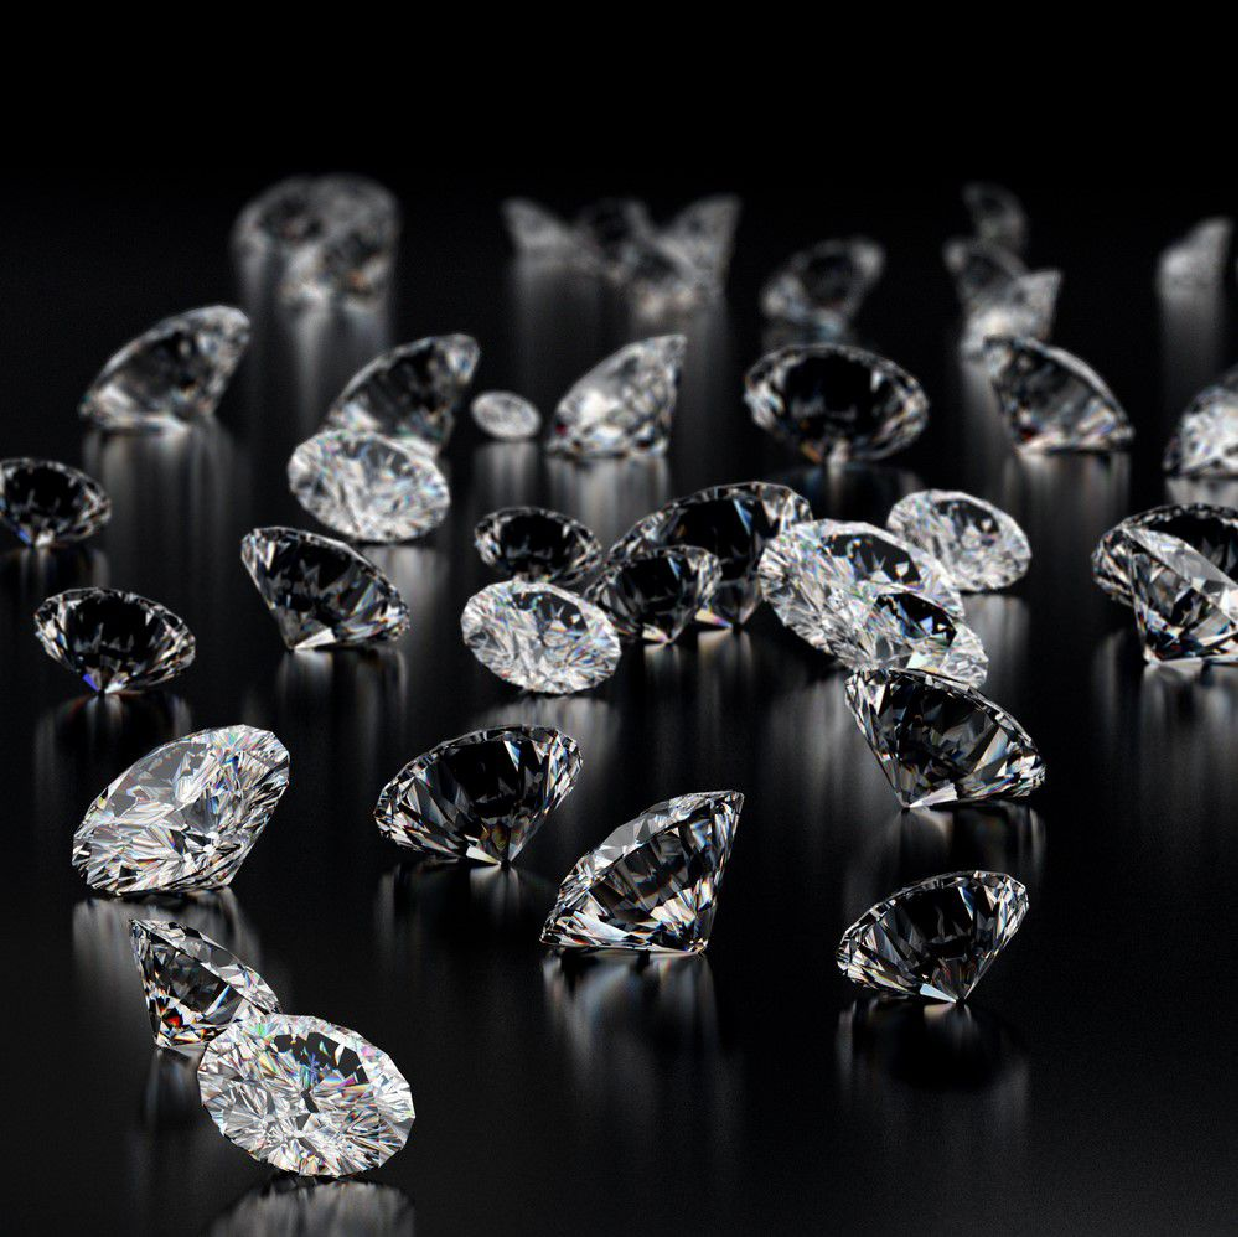
\includegraphics[width=\linewidth]{img/diamond.pdf} 
        \vspace{1ex}
      \end{subfigure}
      \begin{subfigure}[b]{0.49\linewidth}
        \centering
        \includegraphics[width=\linewidth]{img/graphite.pdf} 
        \vspace{1ex}
      \end{subfigure}
    \end{figure}
\end{frame}
\end{comment}

\begin{frame}
    \frametitle{Table of Contents and Goals}
    \tableofcontents
\end{frame}

\begin{frame}
    \frametitle{Structure of Graphene}
    \begin{figure}[H]
        \centering
        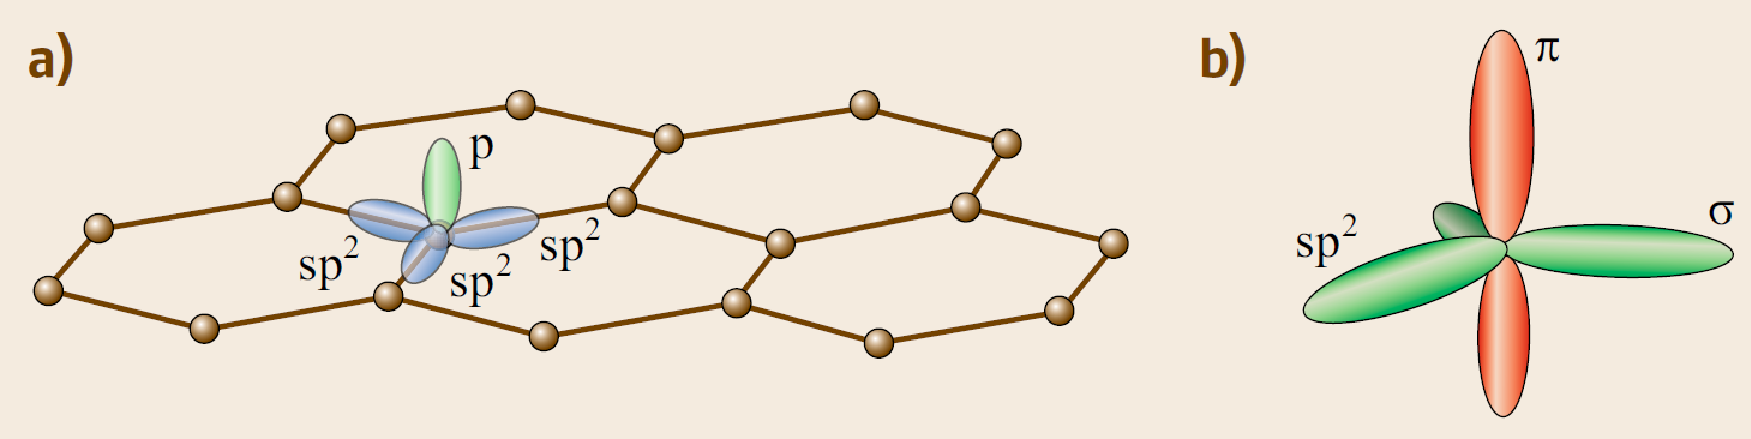
\includegraphics[width=.9\linewidth]{img/graphene_structure.pdf}
    \end{figure}
    \tiny{Image Source: \href{https://link.springer.com/chapter/10.1007/978-3-319-48933-9_48}{10.1007/978-3-319-48933-9\_48}}
\end{frame}

\begin{frame}
    \frametitle{Plasmonics}
    \begin{columns}
    \column{0.5\textwidth}
    \begin{figure}
        \centering
        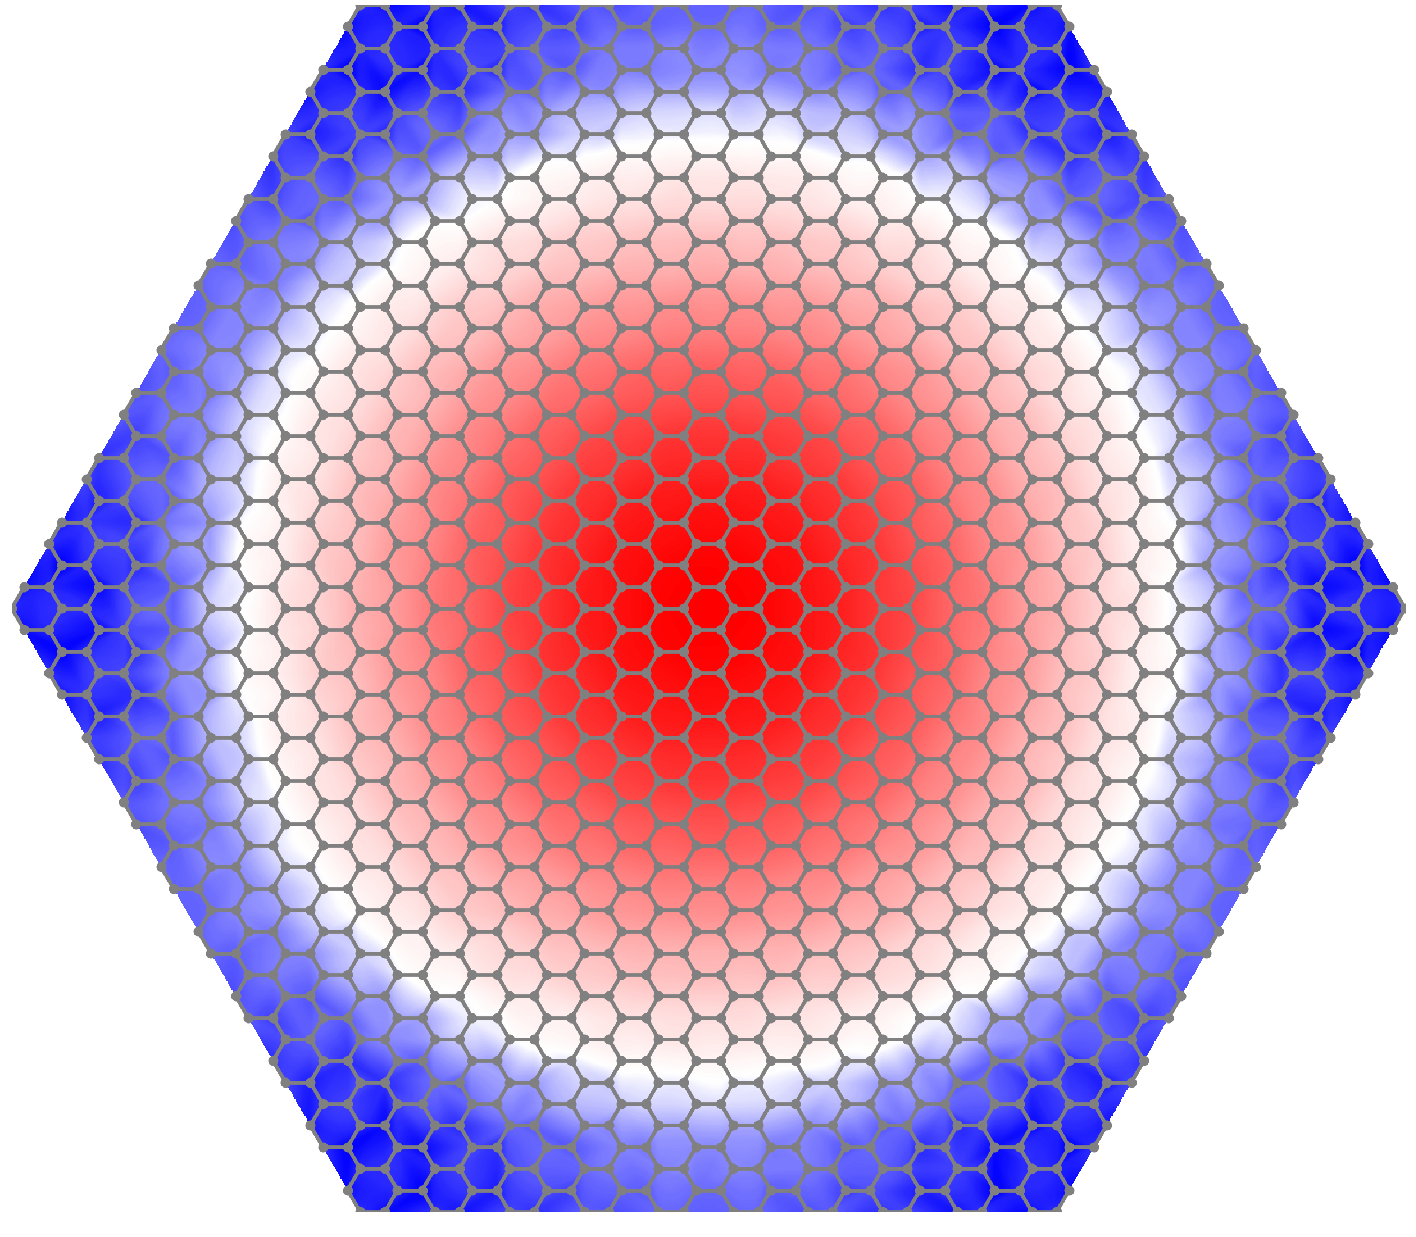
\includegraphics[width=\textwidth]{img/eigenmode.pdf}
    \end{figure}
    \column{0.5\textwidth}
    \begin{itemize}
        \item Plasmons are collective oscillations of charge carriers
        \item Have been studied in metals for some time
        \item As graphene is only one atom thick, it is very sensitive to its environment such that plasmons can be tuned quite easily
    \end{itemize}
    \end{columns}
\end{frame}

\begin{frame}
    \begin{block}{Goals of the Thesis}
     \begin{itemize}
        \item Find Coulomb model which includes screening in real space
        \item Determine real-space plasmonic excitations and investigate their dependency on dielectric screening
    \end{itemize}
    \end{block}
\end{frame}

%%%%%%%%%%%%%%%%%%%%%%%%%%%%%%%%%%

\begin{comment}
\begin{frame}
    \frametitle{Tight-Binding Theory}
    \begin{block}{Hamiltonian}
    \begin{equation}
        \begin{split}
        H &= \sum_{i,j}T_{i,j} c_i^\dagger c_j + \frac{1}{2}\sum_{i,j} U_{i,j} n_i n_j\\
        &= \underbrace{t \sum_{i,j} c_i^\dagger c_j}_{\text{tight-binding matrix}} + \underbrace{\frac{1}{2}\sum_{i,j} U_{i,j} n_i n_j}_{\text{Coulomb interaction matrix}}
        \end{split}
    \end{equation}
    \end{block}
\end{frame}
\end{comment}

\section{Screened Coulomb Interaction}
\begin{frame}
    \frametitle{Screened Coulomb Interaction}
    \begin{figure}
        \centering
        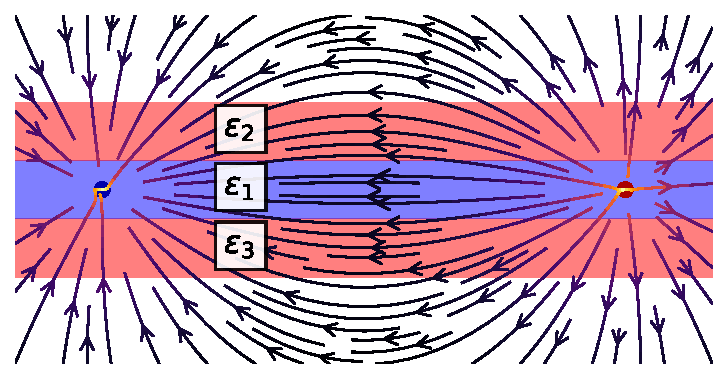
\includegraphics[width=.6\textwidth]{img/FSG_large.pdf}
    \end{figure}
    \begin{block}{Coulomb Interaction assuming $\epsilon_2=\epsilon_3$}
    \begin{equation*}
        U(r)= \underbrace{\frac{e^2}{\epsilon_1 \sqrt{r^2+\delta^2}}}_\ttext{classical} +   \underbrace{\frac{2e^2}{\epsilon_1}\sum_{n=1}^\infty\brackets{\frac{\epsilon_1-\epsilon_2}{\epsilon_1+\epsilon_2}}^{n}\brackets{r^2+\delta^2+n^2h^2}^{-1/2}}_\ttext{screening}
    \end{equation*}
    \end{block}
\end{frame}

%%%%%%%%%%%%%%%%%%%%%%%%%%%%%%%%%%

\begin{frame}
    \frametitle{Free-Standing Graphene}
    \begin{columns}
    \column{0.7\textwidth}
    \begin{figure}[H]
        \centering
        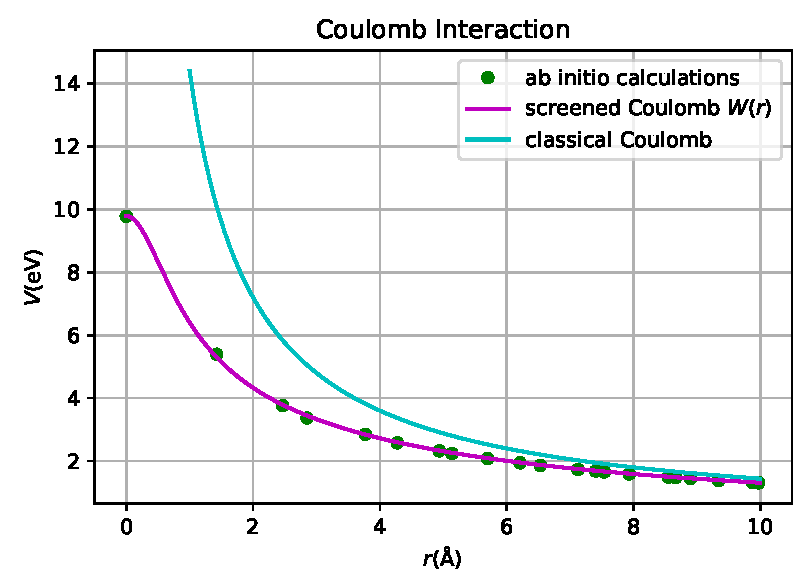
\includegraphics[width=\textwidth]{img/FSG_Cho_2018.pdf}
    \end{figure}
    \column{0.3\textwidth}
    \begin{figure}
        \centering
        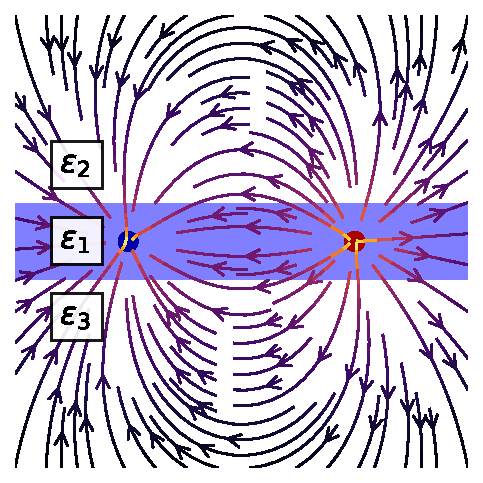
\includegraphics[width=\textwidth]{img/FSG.pdf}
    \end{figure}
    \begin{equation*}
    \begin{split}
        \delta &\approx \SI{0.709}{\angstrom}\\
        \epsilon_1&\approx 2.58\\
        \epsilon_2 &= 1\\
        h &= \SI{3.35}{\angstrom}
    \end{split}
    \end{equation*}
    \end{columns}
\end{frame}

\begin{frame}
    \frametitle{Mono-Layer Graphene Embedded in h-BN}
    \begin{columns}
    \column{0.7\textwidth}
    \begin{figure}[H]
        \centering
        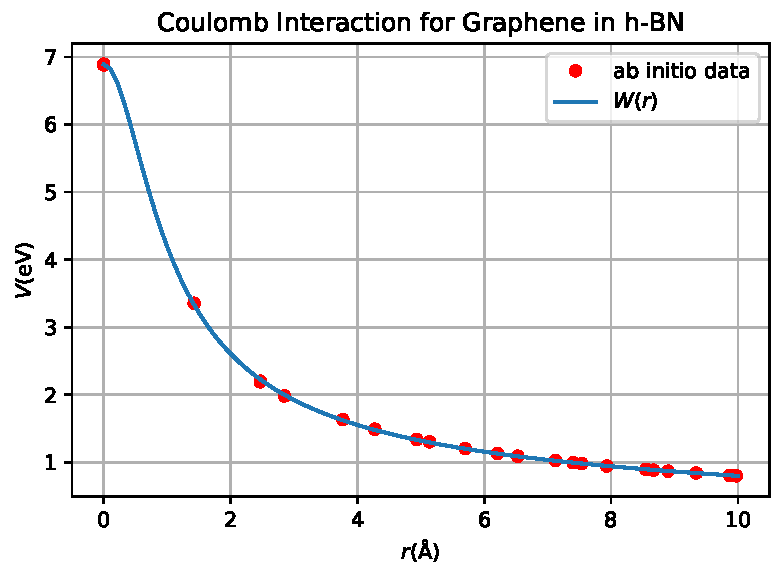
\includegraphics[width=\textwidth]{img/cho_2018_BN_all.pdf}
    \end{figure}
    \column{0.3\textwidth}
        \begin{figure}
        \centering
        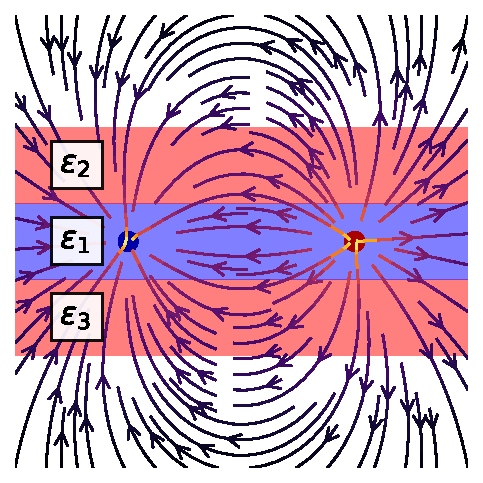
\includegraphics[width=\textwidth]{img/FSG_hBN.pdf}
    \end{figure}
    \begin{equation*}
    \begin{split}
        \delta &\approx \SI{0.716}{\angstrom}\\
        \epsilon_1 &\approx 3.12\\
        \epsilon_2 &\approx 1.34\\
        h &\approx \SI{10.7}{\angstrom}
    \end{split}
    \end{equation*}
    \end{columns}
\end{frame}

%%%%%%%%%%%%%%%%%%%%%%%%%%%%%%%%%%

\section{Plasmons}
\begin{frame}
    \frametitle{Plasmons}
    \begin{block}{Dielectric function}
    \begin{equation}
        \boxed{\begin{rcases}
        (H_\ttext{tb},\omega)\Rightarrow \ttext{RPA} &\Rightarrow \Pi(\omega)\\
        \ttext{ab initio}\Rightarrow \ttext{FT} &\Rightarrow U_{i,j}
        \end{rcases} (\Pi(\omega),U_{i,j}) \Rightarrow \epsilon(\omega) }
    \end{equation}
    \end{block}
\end{frame}

\begin{comment}
\begin{frame}{...}
    \begin{block}{EELS and Eigenmodes}
    \begin{itemize}
        \item The eigenvalues of $\epsilon(\omega)$ can be used to plot the EELS
        \item The peaks of the EELS represent the frequencies at which plasmonic excitations occur
        \item The eigenvectors of $\epsilon(\omega)$ corresponding to the plasmon frequencies are the eigenmodes
    \end{itemize}
    \end{block}
\end{frame}
\end{comment}

\begin{frame}{EELS}
    \begin{figure}
        \centering
        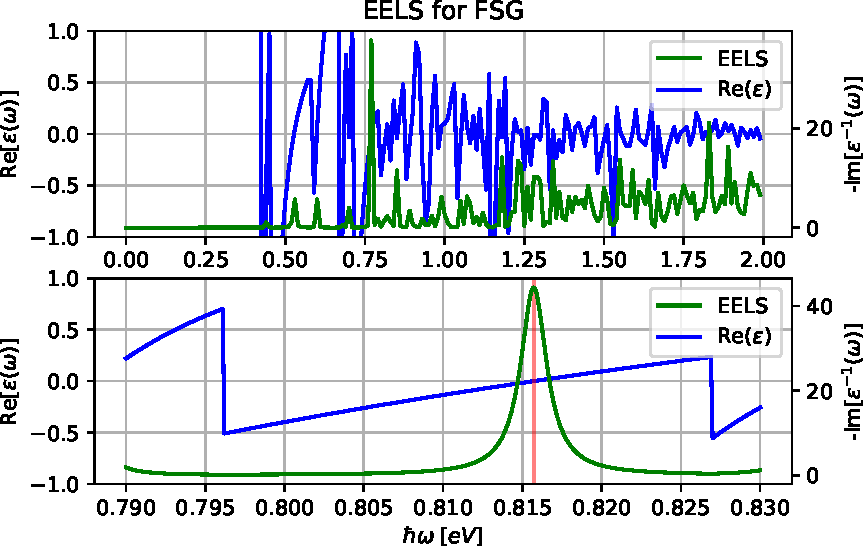
\includegraphics[width=.8\textwidth]{img/eels_FSG_pres.pdf}
    \end{figure}
\end{frame}

\begin{frame}
\frametitle{Eigenmodes for FSG}
\begin{columns}
\column{.5\textwidth}
\begin{figure}[H]
      \begin{subfigure}[b]{0.45\textwidth}
        \centering
        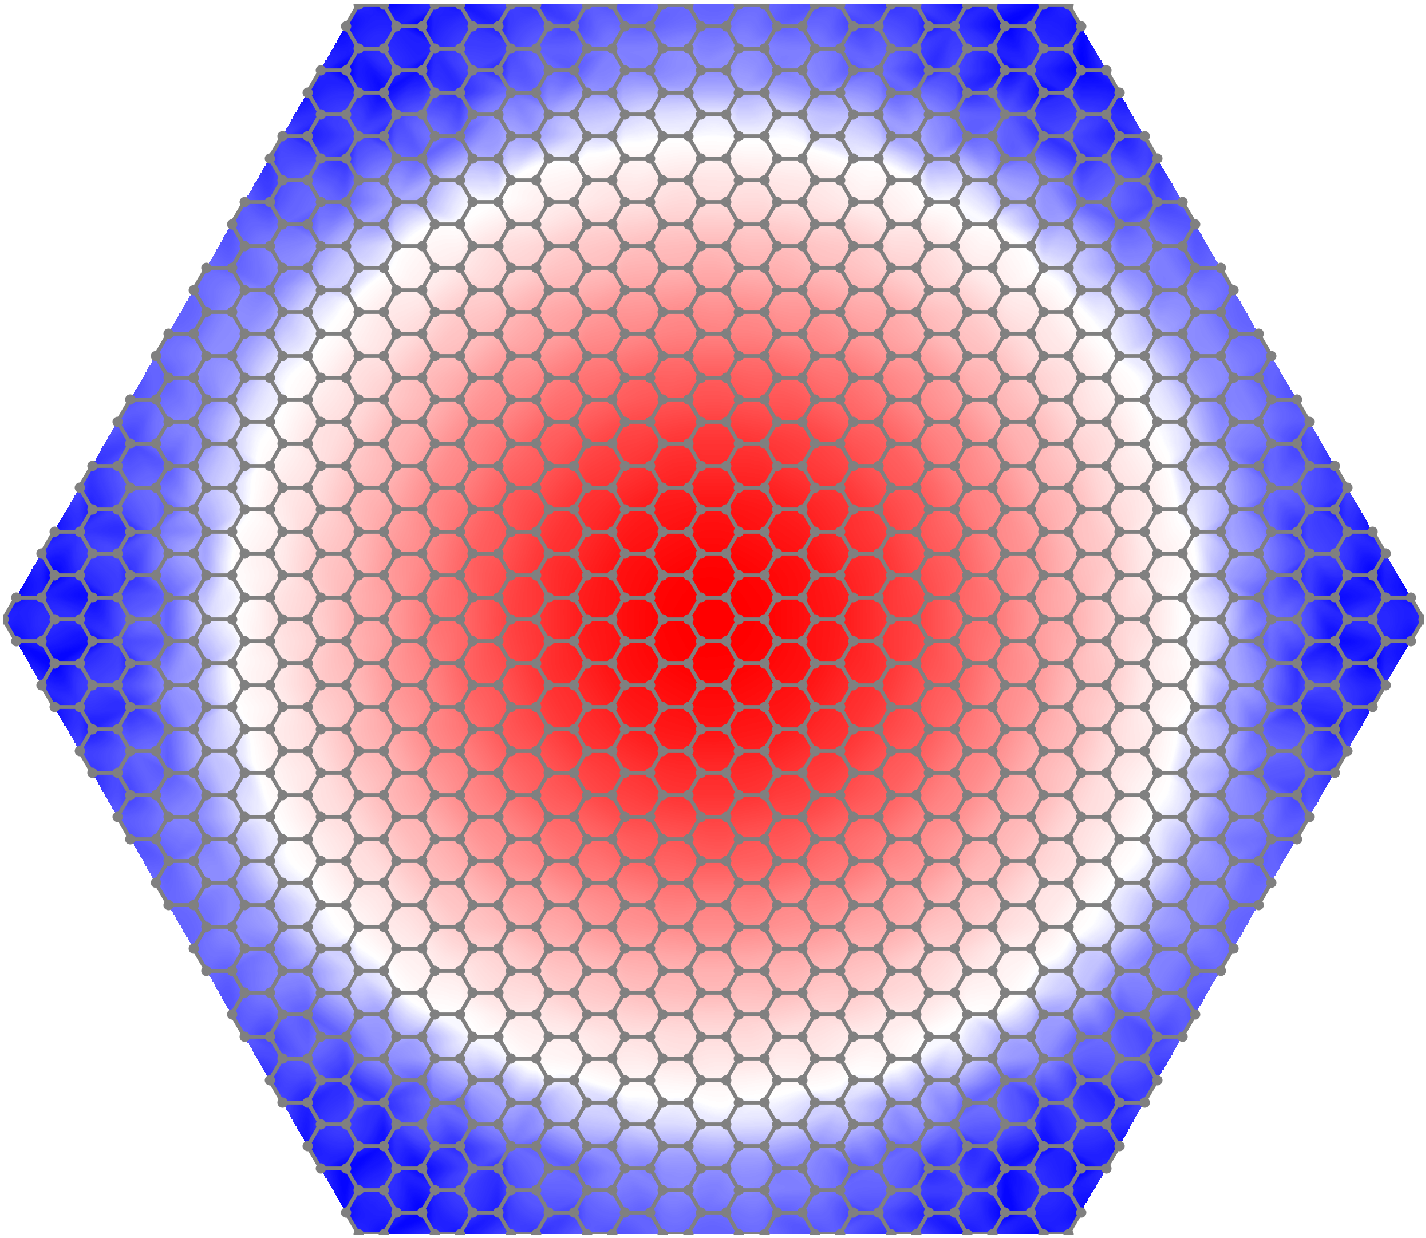
\includegraphics[width=\textwidth]{img/eigenmode_1s.pdf} 
        \caption{1s-like state}
        \vspace{-1ex}
      \end{subfigure}
      \begin{subfigure}[b]{0.45\textwidth}
        \centering
        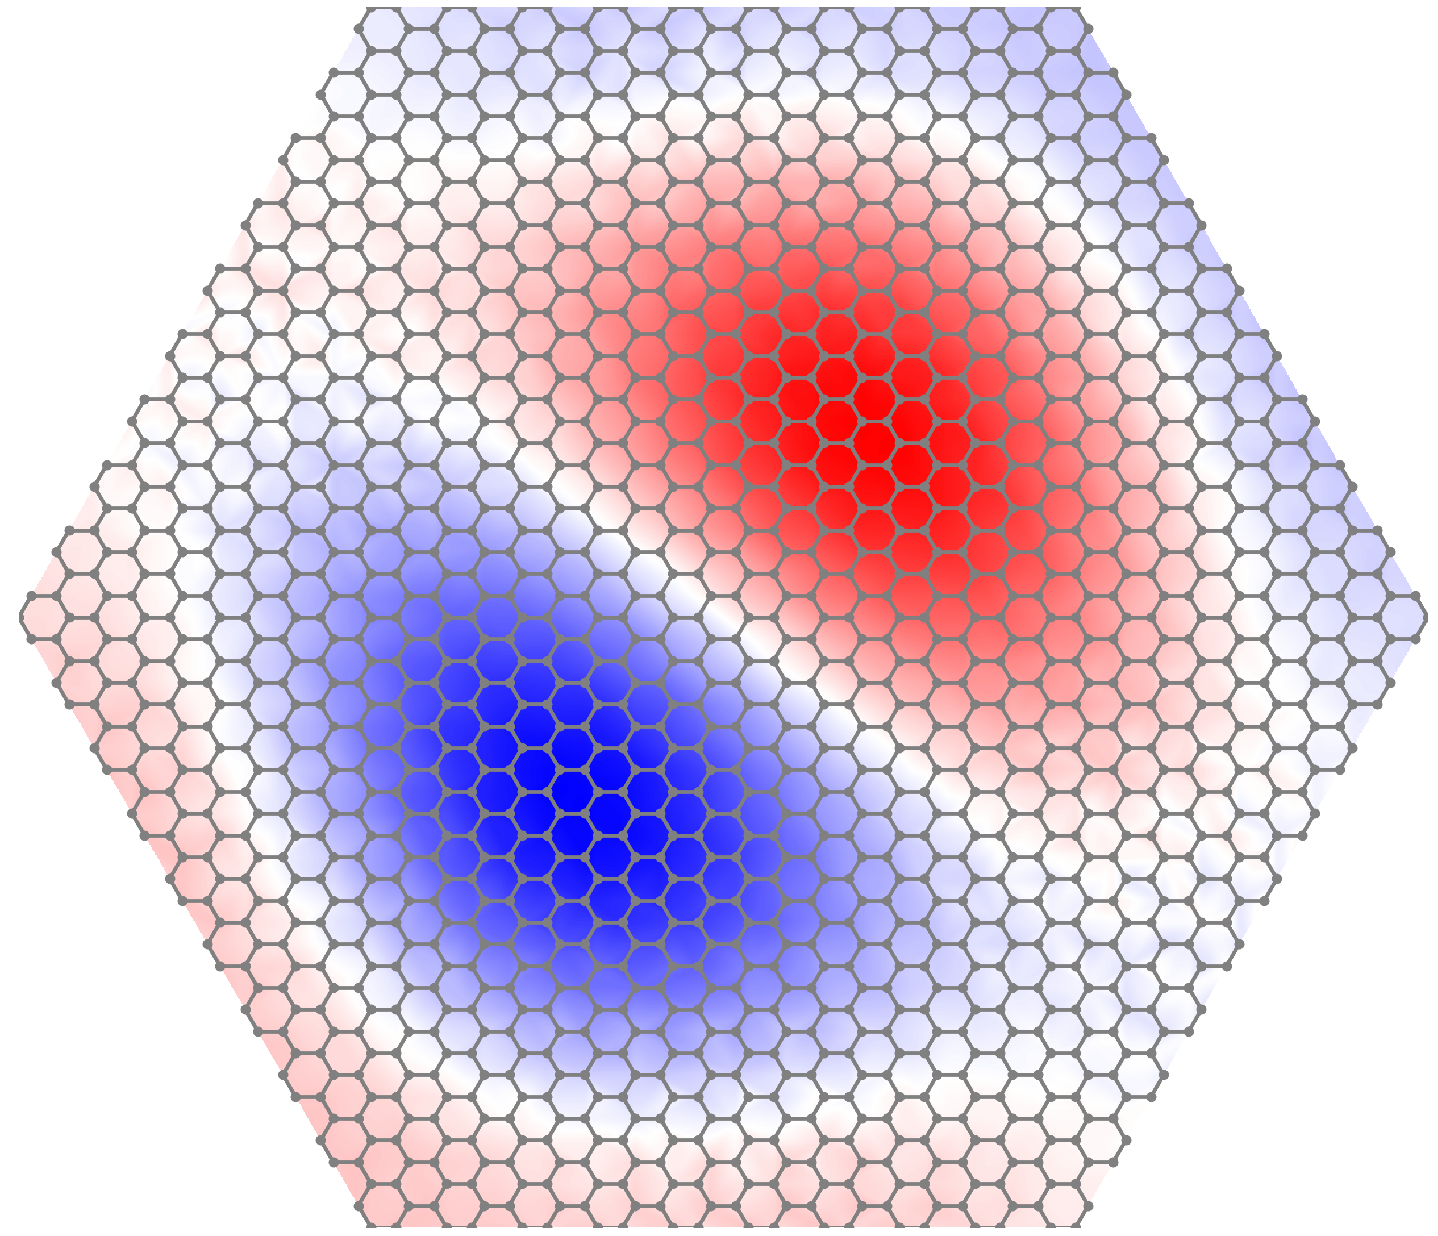
\includegraphics[width=\textwidth]{img/eigenmode_1p.pdf}
        \caption{1p-like state}
        \vspace{-1ex}
      \end{subfigure}
      \begin{subfigure}[b]{0.45\textwidth}
        \centering
        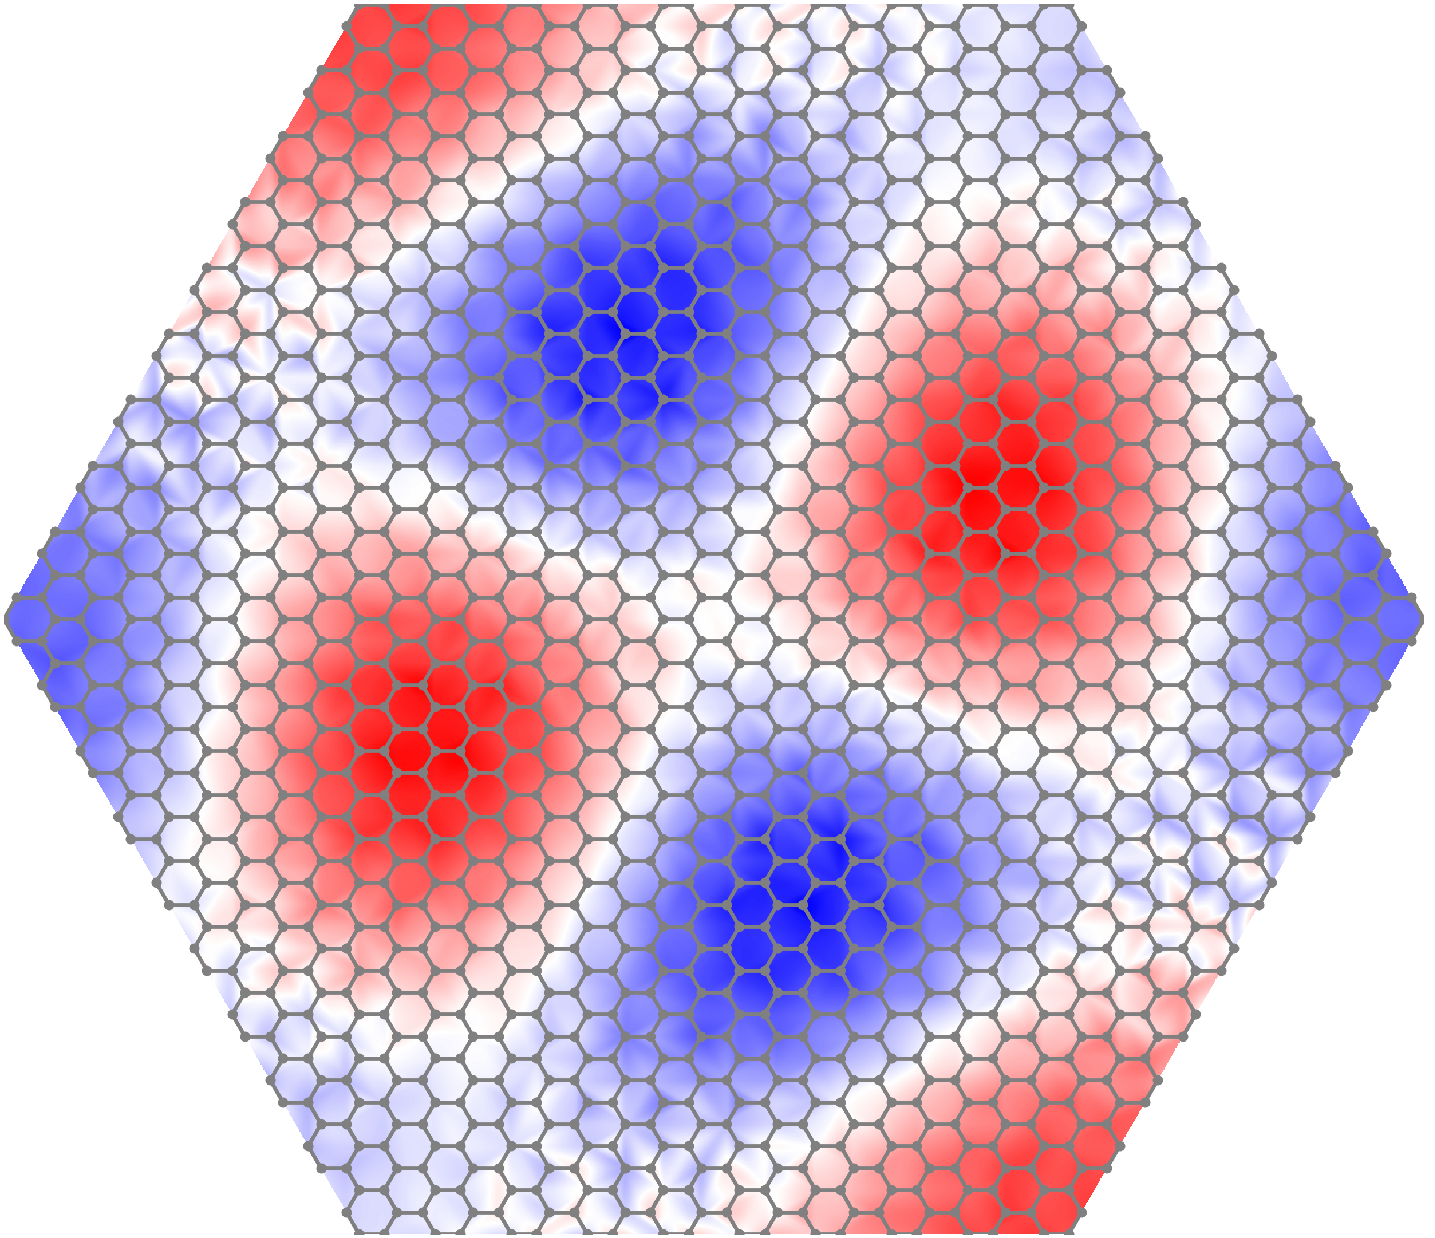
\includegraphics[width=\textwidth]{img/eigenmode_1d.pdf}
        \caption{1d-like state}
        \vspace{-1ex}
      \end{subfigure}
      \begin{subfigure}[b]{0.45\textwidth}
        \centering
        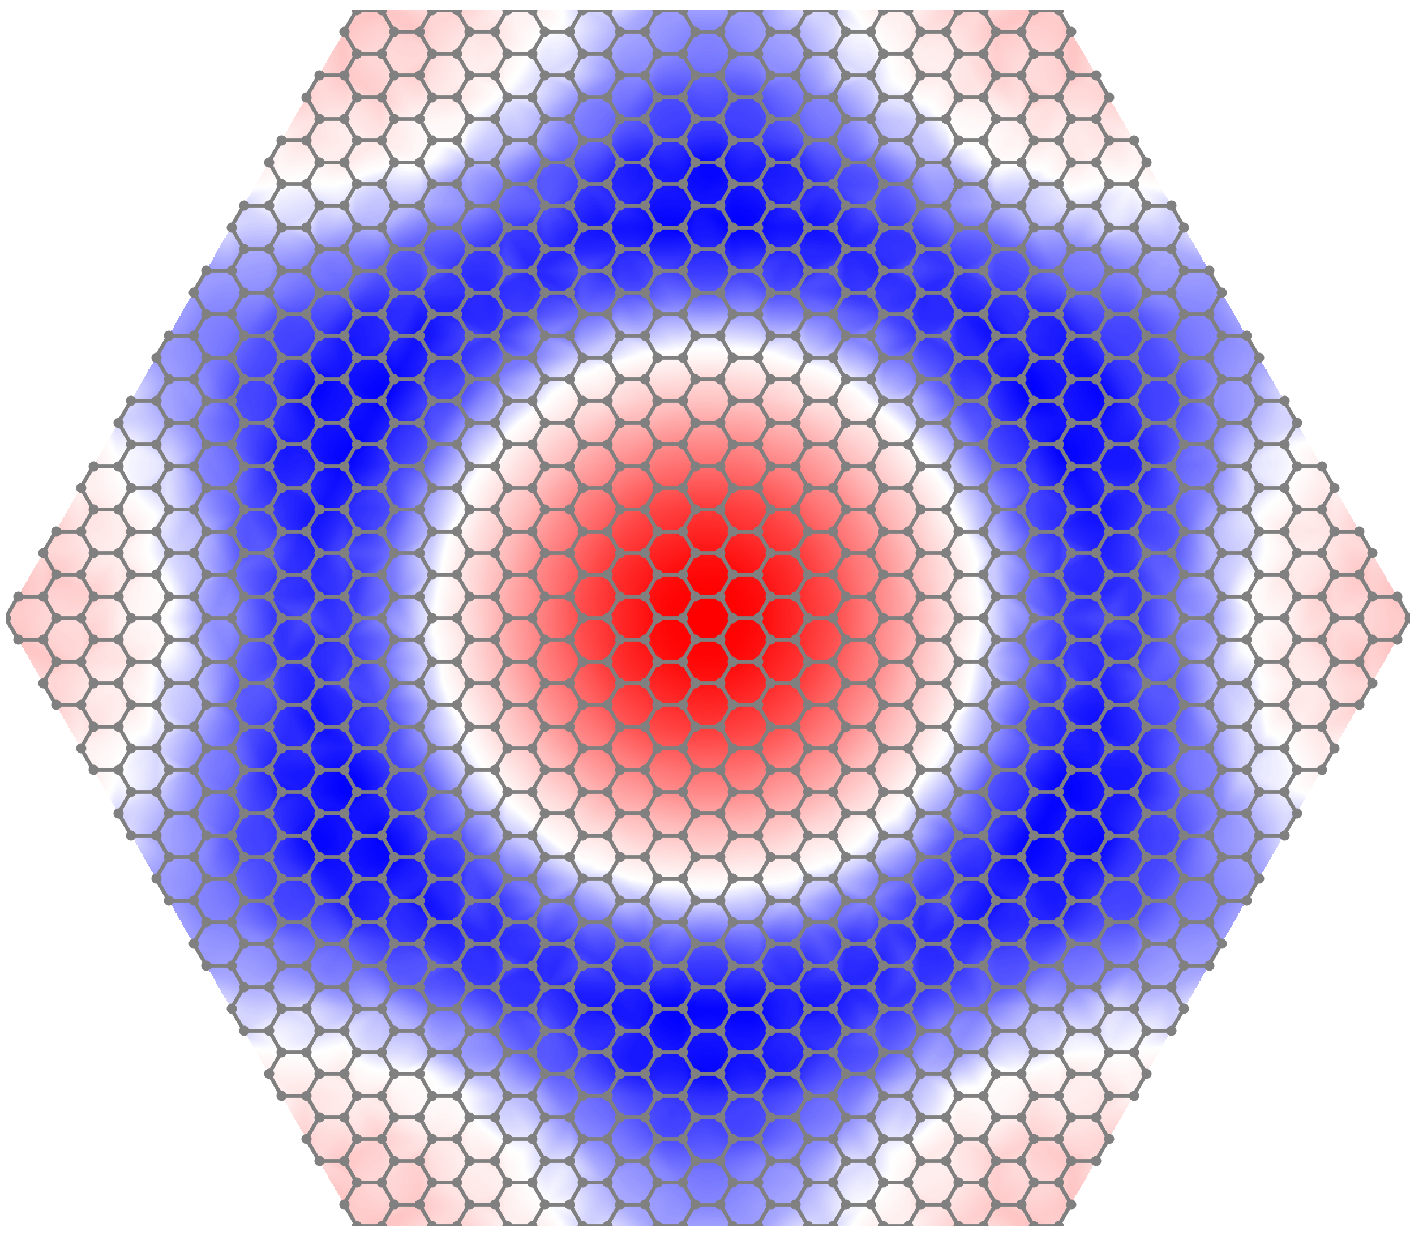
\includegraphics[width=\textwidth]{img/eigenmode_2s.pdf}
        \caption{2s-like state}
        \vspace{-1ex}
      \end{subfigure}
    \end{figure}
\column{.5\textwidth}
\begin{itemize}
    \item Interesting structures where the charge is polarised
    \item Different for h-BN embedding
    \item What is the effect of different dielectric materials?
\end{itemize}
\end{columns}
\end{frame}

\begin{frame}
\frametitle{Different Dielectric Environments}
\begin{columns}
\column{.7\textwidth}
    \begin{figure}[H]
        \centering
        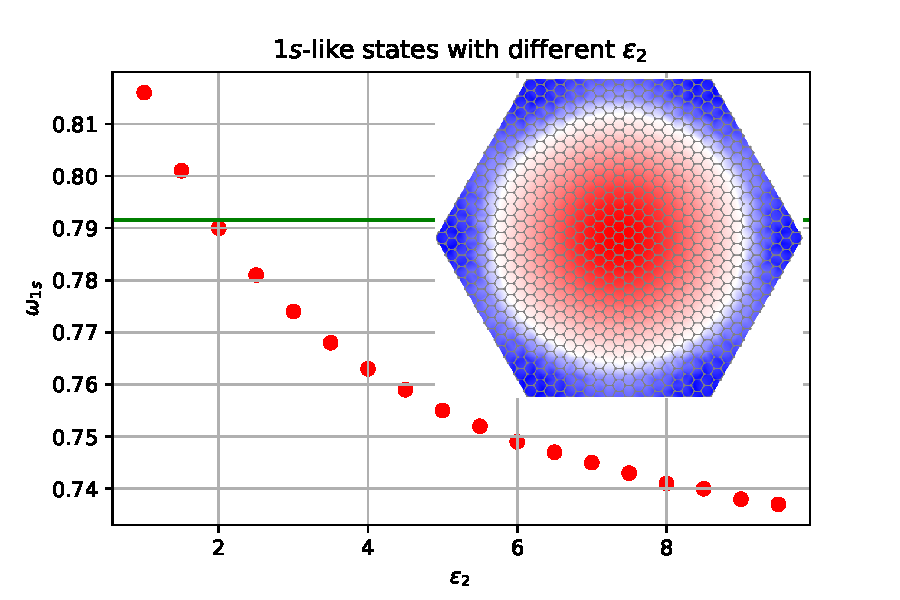
\includegraphics[width=\textwidth]{img/1s.pdf} 
    \end{figure}
\column{.3\textwidth}
\begin{figure}
        \centering
        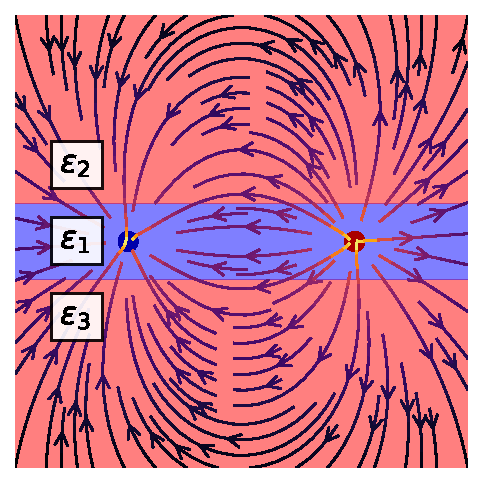
\includegraphics[width=\textwidth]{img/FSG_dielectric.pdf}
    \end{figure}
\end{columns}
\end{frame}

%%%%%%%%%%%%%%%%%%%%%%%%%%%%%%%%

\section{Conclusion and Outlook}
\begin{frame}
  \frametitle{Conclusion and Outlook}
  \begin{itemize}
  \item Results:
  \begin{itemize}
      \item Real-space continuous screened Coulomb interaction model for mono-layer graphene and graphene embedded in h-BN
      \item Plasmon eigenmodes/frequencies depend on the dielectric environment
  \end{itemize}
  \item Further research:
  \begin{itemize}
      \item Analyse parameters for h-BN, new model?
      \item Better tight-binding model
      \item Different substrates
  \end{itemize}
  \end{itemize}
\end{frame}

\end{document}
